\documentclass[]{article}
\usepackage{lmodern}
\usepackage{amssymb,amsmath}
\usepackage{ifxetex,ifluatex}
\usepackage{fixltx2e} % provides \textsubscript
\ifnum 0\ifxetex 1\fi\ifluatex 1\fi=0 % if pdftex
  \usepackage[T1]{fontenc}
  \usepackage[utf8]{inputenc}
\else % if luatex or xelatex
  \ifxetex
    \usepackage{mathspec}
  \else
    \usepackage{fontspec}
  \fi
  \defaultfontfeatures{Ligatures=TeX,Scale=MatchLowercase}
\fi
% use upquote if available, for straight quotes in verbatim environments
\IfFileExists{upquote.sty}{\usepackage{upquote}}{}
% use microtype if available
\IfFileExists{microtype.sty}{%
\usepackage{microtype}
\UseMicrotypeSet[protrusion]{basicmath} % disable protrusion for tt fonts
}{}
\usepackage[margin=1in]{geometry}
\usepackage{hyperref}
\hypersetup{unicode=true,
            pdftitle={Intro Datenanalyse mit R - Dein Freund das GUI},
            pdfauthor={Jan-Philipp Kolb},
            pdfborder={0 0 0},
            breaklinks=true}
\urlstyle{same}  % don't use monospace font for urls
\usepackage{graphicx,grffile}
\makeatletter
\def\maxwidth{\ifdim\Gin@nat@width>\linewidth\linewidth\else\Gin@nat@width\fi}
\def\maxheight{\ifdim\Gin@nat@height>\textheight\textheight\else\Gin@nat@height\fi}
\makeatother
% Scale images if necessary, so that they will not overflow the page
% margins by default, and it is still possible to overwrite the defaults
% using explicit options in \includegraphics[width, height, ...]{}
\setkeys{Gin}{width=\maxwidth,height=\maxheight,keepaspectratio}
\IfFileExists{parskip.sty}{%
\usepackage{parskip}
}{% else
\setlength{\parindent}{0pt}
\setlength{\parskip}{6pt plus 2pt minus 1pt}
}
\setlength{\emergencystretch}{3em}  % prevent overfull lines
\providecommand{\tightlist}{%
  \setlength{\itemsep}{0pt}\setlength{\parskip}{0pt}}
\setcounter{secnumdepth}{0}
% Redefines (sub)paragraphs to behave more like sections
\ifx\paragraph\undefined\else
\let\oldparagraph\paragraph
\renewcommand{\paragraph}[1]{\oldparagraph{#1}\mbox{}}
\fi
\ifx\subparagraph\undefined\else
\let\oldsubparagraph\subparagraph
\renewcommand{\subparagraph}[1]{\oldsubparagraph{#1}\mbox{}}
\fi

%%% Use protect on footnotes to avoid problems with footnotes in titles
\let\rmarkdownfootnote\footnote%
\def\footnote{\protect\rmarkdownfootnote}

%%% Change title format to be more compact
\usepackage{titling}

% Create subtitle command for use in maketitle
\newcommand{\subtitle}[1]{
  \posttitle{
    \begin{center}\large#1\end{center}
    }
}

\setlength{\droptitle}{-2em}
  \title{Intro Datenanalyse mit R - Dein Freund das GUI}
  \pretitle{\vspace{\droptitle}\centering\huge}
  \posttitle{\par}
  \author{Jan-Philipp Kolb}
  \preauthor{\centering\large\emph}
  \postauthor{\par}
  \predate{\centering\large\emph}
  \postdate{\par}
  \date{3 Mai 2017}


\begin{document}
\maketitle

\subsection{Open Source Programm R}\label{open-source-programm-r}

\begin{itemize}
\item
  R ist eine freie, nicht-kommerzielle Implementierung der
  Programmiersprache S (von AT\&T Bell Laboratories entwickelt)
\item
  Freie Beteiligung - modularer Aufbau (immer mehr Erweiterungspakete)
\item
  Der Download ist auf dieser Seite möglich:
\end{itemize}

\url{https://cran.r-project.org/}

\begin{figure}[htbp]
\centering
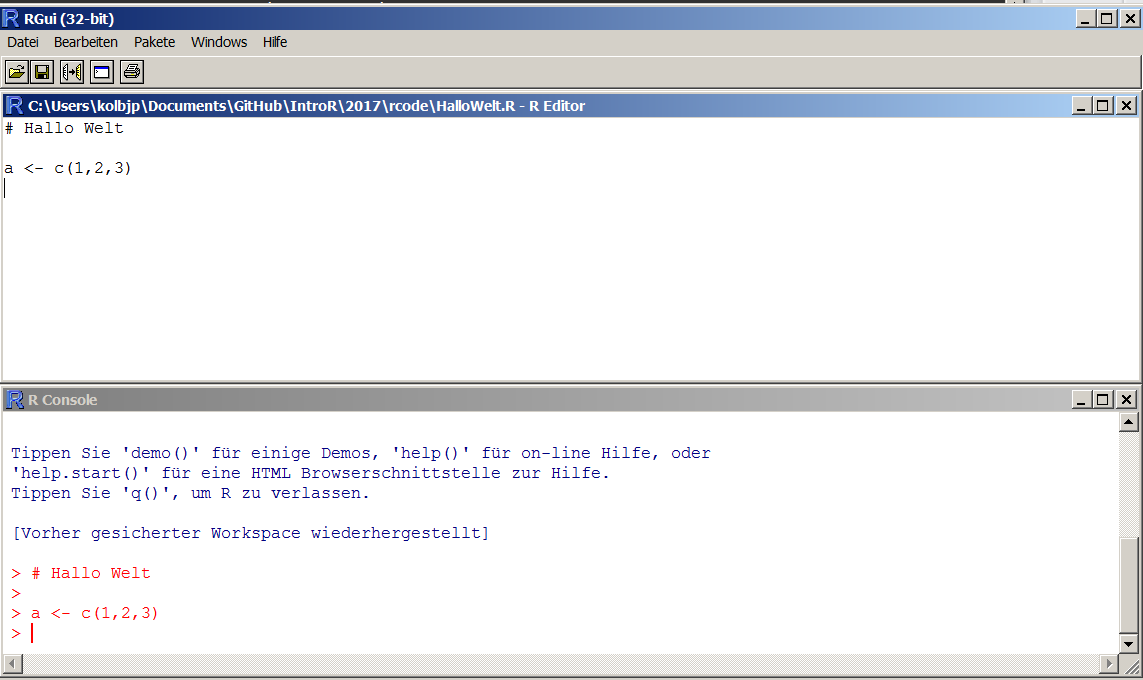
\includegraphics{figure/BasisR.PNG}
\caption{}
\end{figure}

\subsection{Graphisches User
Interface}\label{graphisches-user-interface}

Aber die meisten Menschen nutzen einen Editor oder ein graphical user
interface (GUI).

Aus den folgenden Gründen:

\begin{itemize}
\tightlist
\item
  Syntax highlighting
\item
  Auto-Vervollständigung
\item
  Bessere Übersicht über Graphiken, Bibliotheken
\end{itemize}

\subsection{Verschiedene GUIs}\label{verschiedene-guis}

\begin{itemize}
\item
  \href{https://projects.gnome.org/gedit/}{Gedit} mit R-spezifischen
  Add-ons für Linux
\item
  \href{http://www.gnu.org/software/emacs/}{Emacs}
\item
  \href{http://www.sciviews.org/Tinn-R/}{TinnR}
\item
  Ich nutze \href{https://www.rstudio.com/}{Rstudio!}
\end{itemize}

\begin{figure}[htbp]
\centering
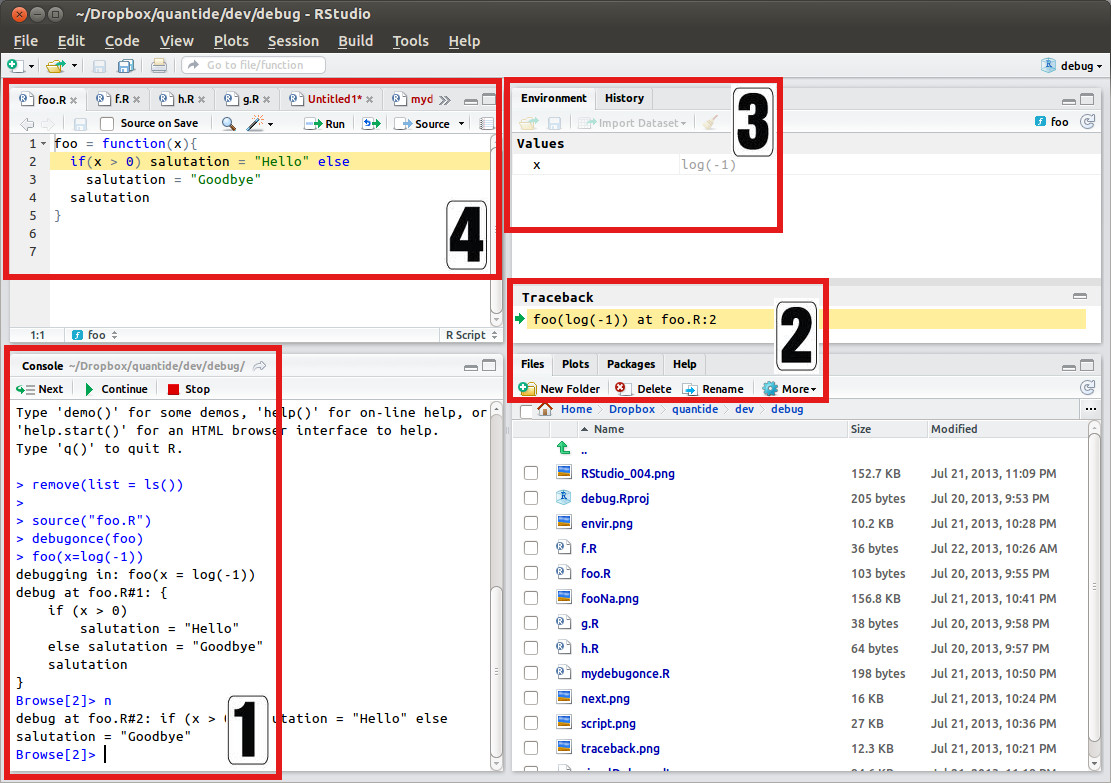
\includegraphics{http://www.milanor.net/blog/wp-content/uploads/2013/07/0_overall.jpg}
\caption{rstudio}
\end{figure}

\subsection{Rstudio}\label{rstudio}

\begin{itemize}
\item
  Sechs
  \href{http://www.r-bloggers.com/top-6-reasons-you-need-to-be-using-rstudio/}{Gründe}
  Rstudio zu nutzen.
\item
  Wie man Rstudio
  \href{https://support.rstudio.com/hc/en-us/sections/200107586-Using-RStudio}{nutzen
  kann.}
\item
  \href{https://support.rstudio.com/hc/en-us/articles/200549016-Customizing-RStudio}{Das
  Rstudio einrichten}
\end{itemize}

\subsection{Download der Unterlagen}\label{download-der-unterlagen}

Auf \href{https://github.com/Japhilko/IntroR/tree/master/2017}{github}
sind alle Unterlagen für diesen Kurs zu finden.

\href{https://guides.github.com/activities/hello-world/}{Wie nutzt man
github?}


\end{document}
